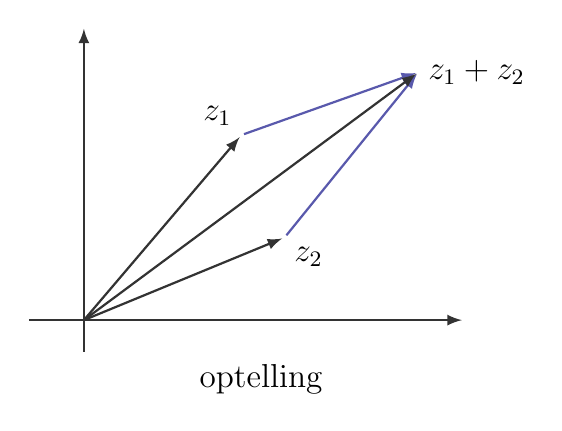
\begin{tikzpicture}[>=latex]

% --- Global TikZ Styles ---
\tikzset{
    axis/.style={
        ->,
        >=latex,
        thick,
        draw=black!80
    },
    vector/.style={
        ->,
        >=latex,
        thick,
        draw=black!80,
        shorten >=1pt
    },
    helper/.style={
        ->,
        >=latex,
        thick,
        draw=NavyBlue!65,
        shorten >=1pt,
        shorten <=1pt
    },
    element/.style={
        font=\large
    }
}

% ==================================================
% --- Assen ---
% ==================================================

\draw[axis] (-0.7,0) -- (4.8,0);
\draw[axis] (0,-0.4) -- (0,3.7);

% ==================================================
% --- Coördinaten ---
% ==================================================

\coordinate (O) at (0,0);
\coordinate (zone) at (2.0,2.35);
\coordinate (ztwo) at (2.55,1.05);
\coordinate (zsum) at (4.25,3.15);

% ==================================================
% --- Vectoren ---
% ==================================================

% z_1 en z_2 vanuit de oorsprong
\draw[vector] (O) -- (zone);
\draw[vector] (O) -- (ztwo);

% Kleine hulpvectoren zoals in de schets
\draw[helper] (ztwo) -- (zsum);
\draw[helper] (zone) -- (zsum);

% z_1 + z_2 vanuit de oorsprong
\draw[vector] (O) -- (zsum);

% ==================================================
% --- Labels ---
% ==================================================

\node[element, anchor=south east] at (zone) {$z_1$};
\node[element, anchor=north west] at (ztwo) {$z_2$};
\node[element, anchor=west] at (zsum) {$z_1 + z_2$};

\node[element] at (2.25,-0.75) {optelling};

\end{tikzpicture}